\documentclass[12pt]{article}
\usepackage{amsmath}
\usepackage{graphicx}
\usepackage{tikz}
\usepackage{pgfplots}

\title{Plotting\\an Equation\\on a Graph}\\
\author{Tutoring Centre Ferndale\\

\includegraphics[width=4em]{ApS_logo.png}}
\date{}\\

\begin{document}

\maketitle

In algebra, an equation describes a relationship between variables. These variables can be plotted in a table and visualized as a line on a graph.

\section*{Axes and Dimensions}

\begin{itemize}
    \item An axis is a line used to measure relative position. The Earth turns around an axis, for example, and navigation is done by measuring distances from that line. In maths, an axis is a line against which a distance can be measured in some direction. The plural of axis is axes, pronounced "ax-ees." Axes are usually marked with lines along them, called ticks, and numbers, like a ruler.
    \item Dimensions are possible directions of movement, each with a corresponding axis. Each dimensions can be measured by a single number, such as length or width or height.

\newpage

\section*{Dependent and Independent Variables}

In an equation, the independent variable is the one you choose or control, while the dependent variable depends on the value of the independent variable.

For example, in the equation \( y = 2x + 1 \), \( x \) is the independent variable and \( y \) is the dependent variable.

\begin{itemize}
    \item Substituting $x=1$ into $y=2x+1$ gives $y=2\cdot1+1=3$.
    \item Substituting $x=2$ into $y=2x+1$ gives $y=2\cdot5+1=5$.
    \item Each value of $y$ depends on the given value of $x$.
\end{itemize}

Here is a table of different integer values of $y$ for different values of $x$ between -2 and 2:

\vspace{24pt}

\begin{center}
\resizebox{0.5\textwidth}{!}{
\begin{tabular}{|c|c|c|c|c|c|}
\hline
$x$ & -2 & -1 & 0 & 1 & 2 \\
\hline
$y$ & -3 & -1 & 1 & 3 & 5 \\
\hline
\end{tabular}
}
\par\vspace{1em}
\Large{$y=2x+1$}
\end{center}

\newpage

\section*{Graphing 2 Dimensions}
\item A flat graph has two axes: the horizontal axis ($x$-axis) and the vertical axis ($y$-axis). These axes represent the dimensions of the graph. The independent variable is plotted on the $x$-axis, and the dependent variable is plotted on the $y$-axis.
\item The point where the axes meet at zero is called the origin.
\end{itemize}

\vspace{24pt}

\begin{center}
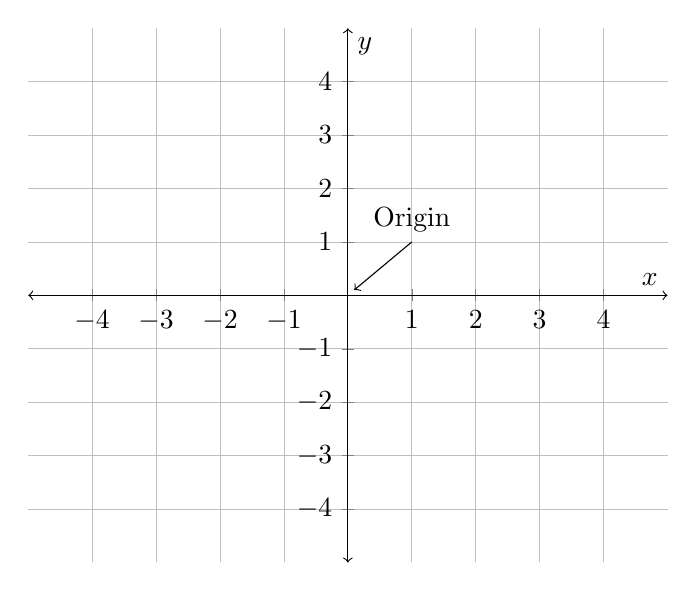
\begin{tikzpicture}
    \begin{axis}[
        width=0.8\textwidth,
        axis lines = middle,
        axis line style={<->},
        xlabel = $x$,
        ylabel = $y$,
        xmin=-5, xmax=5,
        ymin=-5, ymax=5,
        xtick={-4,-3,...,4},
        ytick={-4,-3,...,4},
        grid=both,
        grid style={line width=.3pt, draw=gray!50}]
    \draw[<-] (axis cs:.1,.1) -- (axis cs:1,1) node[above] {Origin};
\end{axis}
\end{tikzpicture}
\end{center}

\newpage

\section*{Cartesian Coordinates}

Each pair of values (x, y) represents a point on the graph, known as Cartesian coordinates.

\begin{itemize}
    \item To coordinate means to work with someone or something else. Coordinates in maths are sets of numbers that work together to mark an exact location.
    \item Sets of numbers used this way are called Cartesian coordinates. They are named after the French mathematician and philosopher Renee Descartes who wrote about them in an important book in 1637. His book popularized the idea of coordinates and made it possible to use algebra to solve problems of geometry.
\end{itemize}

Earlier we made a table by substituting values of \( x \) into the equation \( y = 2x + 1 \)to find corresponding values of \( y \). We can now plot these as Cartesian coordinates onto a pair of axes.

\begin{center}
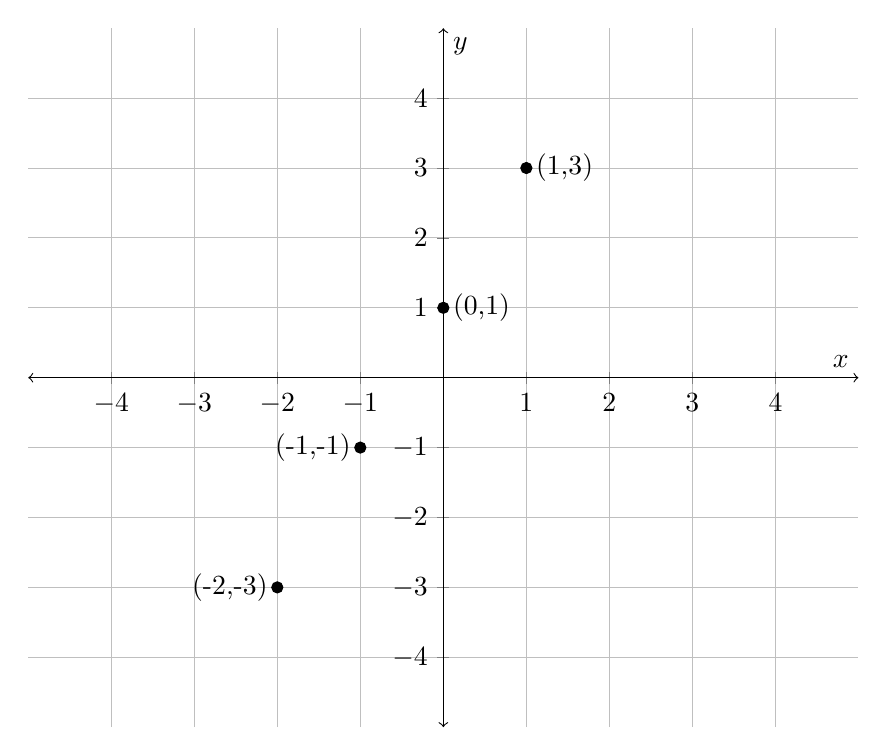
\begin{tikzpicture}
    \begin{axis}[width=\textwidth,
                 axis lines = middle,
                 axis line style={<->},
                 xlabel = $x$,
                 ylabel = $y$,
                 xmin=-5, xmax=5,
                 ymin=-5, ymax=5,
                 xtick={-4,-3,...,4},
                 ytick={-4,-3,...,4},
                 grid=both,
                 grid style={line width=.3pt, draw=gray!50}]
    \addplot[only marks, mark=*]
    coordinates {(-2,-3) (-1,-1) (0,1) (1,3)};
    \node at (axis cs:-2,-3) [anchor=east] {(-2,-3)};
    \node at (axis cs:-1,-1) [anchor=east] {(-1,-1)};
    \node at (axis cs:0,1) [anchor=west] {(0,1)};
    \node at (axis cs:1,3) [anchor=west] {(1,3)};
    \end{axis}
\end{tikzpicture}
\end{center}

\newpage

\section*{Plotting the Line}

Drawing a line through these plotted points will give us all possible values of $x$ and $y$ that satisfy the equation $y=2x+1$.

\begin{itemize}
    \item The plotted line can have an arrow at each end to show that it continues forever in both directions.
    \item The equation should be written along the line as a label or below or beside the graph.
\end{itemize}

\begin{center}
\begin{tikzpicture}[domain/.style={domain, very thick, smooth}]
    \draw[<->] (-5,0) -- (5,0) node[right] {$x$};
    \draw[<->] (0,-5) -- (0,5) node[above] {$y$};
    \foreach \x in {1,...,4}
	\draw (\x,4pt) -- +(0,-8pt) node [below] {$\x$};
    \foreach \x in {-4,...,-1}
	\draw (\x,4pt) -- +(0,-8pt) node [below] {$\x$};
    \foreach \y in {1,...,4}
	\draw (4pt,\y) -- +(-8pt,0) node [left] {$\y$};
    \foreach \y in {-4,...,-1}
	\draw (4pt,\y) -- +(-8pt,0) node [left] {$\y$};
        \draw[domain, thick, <->] (-2,-3) -- (2,5) 
    node[pos=0.85, sloped, below] {$y=2x+1$};
    \foreach \x in {-4,...,4} \draw[width=.3pt, draw=gray!50] (\x,-5) -- (\x,5);
    \foreach \y in {-4,...,4} \draw[width=.3pt, draw=gray!50] (-5,\y) -- (5,\y);
\end{tikzpicture}
\end{center}

The independent variable is plotted on the x-axis, and the dependent variable is plotted on the y-axis. Each point on the graph represents a pair of values, and the line shows the continuous relationship defined by the equation.

Any equation in algebra can be plotted in a graph this way. Plotting an equation helps to visualize the relationship between variables and can be used to solve many practical problems of geometry.

\end{document}
